\newcommand{\halfangle}{10}
\newcommand{\dr}{.3 cm}
\newcommand{\rbeg}{1.5 cm}
\newcommand{\Larrow}{.25 cm}
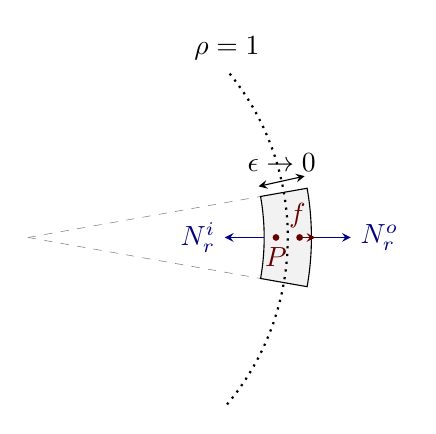
\begin{tikzpicture}[scale=2]
	%The bisected dotted lines
	\begin{scope}[dashed,gray,very thin]
		\draw (0,0) -- (\halfangle:\rbeg);
		\draw (0,0) -- (-\halfangle:\rbeg);
	\end{scope}
	%Draw the area element
	\filldraw[fill=gray!10,draw=black] (-\halfangle:\rbeg)  arc(-\halfangle:\halfangle:\rbeg) -- (\halfangle:\rbeg+\dr) arc(\halfangle:-\halfangle:\rbeg+\dr) -- cycle;
	%Draw the edge of the hole
	\draw[dotted,thick] (-4*\halfangle:\rbeg+\dr/2) arc(-4*\halfangle:4*\halfangle:\rbeg+\dr/2) node[anchor=south]{$\rho=1$};
	%Draw the force lines and labels
	\begin{scope}[->, blue!50!black,>=stealth]
		\draw (0:\rbeg+\dr) -- +(0:\Larrow) node[anchor=west]{$N_r^o$};
		\draw (0:\rbeg) -- +(0:-\Larrow) node[anchor=east]{$N_r^i$};
		\filldraw[red!40!black] (\rbeg+\dr*3/4,0) circle(.5pt);
		\draw[red!40!black] (\rbeg+\dr*3/4,0) -- +(.1,0) node[anchor=south east]{$f$};
		\filldraw[red!40!black] (\rbeg+\dr*1/4,0) circle(.5pt) node[anchor=north]{$P$};
	\end{scope}
	%Draw the width of the element
	\draw[<->,black,>=stealth] (\halfangle*5/4:\rbeg) -- node[anchor=south]{$\epsilon \rightarrow 0$} +(\halfangle*5/4:\dr);
\end{tikzpicture}